\begin{frame}{Cubbit}
\centering

\includegraphics[width=0.4\linewidth]{static/cubbit-logo.png}
\\
\vspace{1em}
Cubbit, a geo-distributed storage system.\\
\end{frame}

\begin{frame}{Cubbit -- How it works}
    \begin{columns}[c]
        \begin{column}{0.4\textwidth}
            Each file is split into $n+k$ pieces (i.e., \textbf{shards}) using
            Reed-Solomon. Each shard is sent to a different node (i.e., \textbf{agent}). \\ At least $n$ shards are
            required to reconstruct the file, while $k$ shards provide redundancy.
        \end{column}
        \begin{column}{0.6\textwidth}

            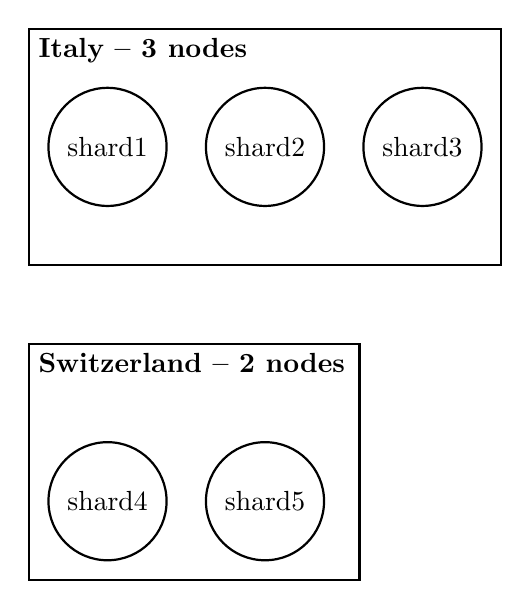
\begin{tikzpicture}
                \draw[thick] (0,0) rectangle (4.2,3);
                \node[anchor=north west] at (0,3) {\textbf{Switzerland -- 2 nodes}};
                \node[circle, draw, thick, minimum size=1.5cm] at (1,1) {shard4};
                \node[circle, draw, thick, minimum size=1.5cm] at (3,1) {shard5};

                \draw[thick] (0,4) rectangle (6,7);
                \node[anchor=north west] at (0,7) {\textbf{Italy -- 3 nodes}};
                \node[circle, draw, thick, minimum size=1.5cm] at (1,5.5) {shard1};
                \node[circle, draw, thick, minimum size=1.5cm] at (3,5.5) {shard2};
                \node[circle, draw, thick, minimum size=1.5cm] at (5,5.5) {shard3};
            \end{tikzpicture}
        \end{column}
    \end{columns}
\end{frame}

\begin{frame}{Cubbit -- Problems using checksum}
    \begin{columns}[c]
        \begin{column}{0.4\textwidth}
            \begin{enumerate}
                \item<1-> If nodes are offline, it becomes impossible to check all shards for a file.
                \item<2-> During upload, some \textbf{nodes may be offline}, but they might be online during verification.
                \item<3-> Should we check each reconstructed file or each shard individually?
            \end{enumerate}

        \end{column}
        \begin{column}{0.6\textwidth}

            \begin{tikzpicture}
                \draw[thick] (0,0) rectangle (4.2,3);
                \node[anchor=north west] at (0,3) {\textbf{Switzerland -- 2 nodes}};
                \node[circle, draw, dotted, minimum size=1.5cm] at (1,1) {shard4};
                \node[circle, draw, dotted, minimum size=1.5cm] at (1,1) {shard4};
                \node[circle, draw, thick, minimum size=1.5cm] at (3,1) {shard5};

                \draw[thick] (0,4) rectangle (6,7);
                \node[anchor=north west] at (0,7) {\textbf{Italy -- 3 nodes}};
                \node[circle, draw, thick, minimum size=1.5cm] at (1,5.5) {shard1};
                \only<1>{\node[circle, draw, thick, minimum size=1.5cm] at (3,5.5) {shard2};}
                \only<2->{\node[circle, draw, thick, minimum size=1.5cm] at
                (3,5.5) {n/a};}
                \node[circle, draw, dotted, minimum size=1.5cm] at (5,5.5) {shard3};
            \end{tikzpicture}
        \end{column}
    \end{columns}
\end{frame}
